 
\begin{center}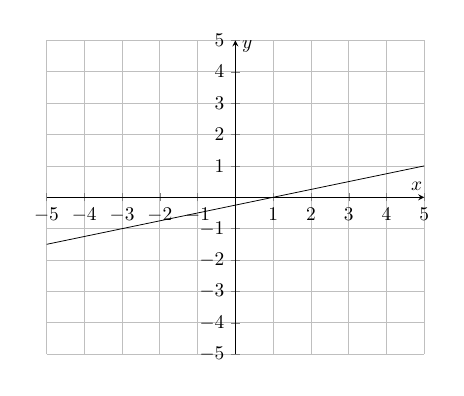
\begin{tikzpicture}[scale=0.7]\begin{axis}[axis lines=center, grid=both, xtick={-5, -4, ..., 5}, ytick={-5, -4, ..., 5},ymin=-5,ymax=5,]
\addplot[samples=4, domain=-5:5]{x/4-1/4};
\draw(axis cs:4.8,0)node[anchor=south]{$x$};
\draw(axis cs:0,4.8)node[anchor=west]{$y$};
\end{axis}\end{tikzpicture}\end{center}
What is the slope of the line in the graph above?\\\\


\ifsat
	\begin{enumerate}[label=\Alph*)]
	\end{enumerate}
\else
\fi

\ifacteven
	\begin{enumerate}[label=\textbf{\Alph*.},itemsep=\fill,align=left]
		\setcounter{enumii}{5}
		\item None of these. 
	\end{enumerate}
\else
\fi

\ifactodd
	\begin{enumerate}[label=\textbf{\Alph*.},itemsep=\fill,align=left]
		\item None of these. 
	\end{enumerate}
\else
\fi

\ifgridin
$\frac{1}{4}$ or $.25$
\else
\fi

